\documentclass[a4paper,11pt]{book}
%\documentclass[a4paper,twoside,11pt,titlepage]{book}
\usepackage{listings}
\usepackage[utf8]{inputenc}
\usepackage{url}
\usepackage[spanish,es-tabla]{babel}

\usepackage{amsmath}
\usepackage{array}
\usepackage{booktabs}
\usepackage{tabulary}
\usepackage{multirow}



\makeatletter
\def\BState{\State\hskip-\ALG@thistlm}
\makeatother

% \usepackage[style=list, number=none]{glossary} %
%\usepackage{titlesec}
%\usepackage{pailatino}

\decimalpoint
\usepackage{dcolumn}
\newcolumntype{.}{D{.}{\esperiod}{-1}}
\makeatletter
\addto\shorthandsspanish{\let\esperiod\es@period@code}
\makeatother


%\usepackage[chapter]{algorithm}
\RequirePackage{verbatim}
%\RequirePackage[Glenn]{fncychap}
\usepackage{fancyhdr}
\usepackage{graphicx}
\usepackage{afterpage}

\usepackage{longtable}

\usepackage[pdfborder={0 0 0}]{hyperref}

% ********************************************************************
% Re-usable information
% ********************************************************************
\newcommand{\myTitle}{Sistemas de recomendación a grupos\xspace}
\newcommand{\myMaster}{Máster en Ciencia de Datos e Ingeniería de Computadores\xspace}
\newcommand{\myName}{Juan José Sierra González\xspace}
\newcommand{\myProf}{Juan Manuel Fernández Luna\xspace}
\newcommand{\myFaculty}{Escuela Técnica Superior de Ingenierías Informática y de
Telecomunicación\xspace}
\newcommand{\myFacultyShort}{E.T.S. de Ingenierías Informática y de
Telecomunicación\xspace}
\newcommand{\myDepartment}{Departamento de Ciencias de la Computación e Inteligencia Artificial\xspace}
\newcommand{\myUni}{\protect{Universidad de Granada}\xspace}
\newcommand{\myLocation}{Granada\xspace}
\newcommand{\myTime}{\today\xspace}
\newcommand{\myVersion}{Version 0.1\xspace}


\hypersetup{
pdfauthor = {\myName (email (en) ugr (punto) es)},
pdftitle = {\myTitle},
pdfsubject = {},
pdfkeywords = {palabra_clave1, palabra_clave2, palabra_clave3, ...},
pdfcreator = {LaTeX con el paquete ....},
pdfproducer = {pdflatex}
}

%\hyphenation{}


%\usepackage{doxygen/doxygen}
%\usepackage{pdfpages}
\usepackage{url}
\usepackage{colortbl,longtable}
\usepackage[stable]{footmisc}
%\usepackage{index}

%\makeindex
%\usepackage[style=long, cols=2,border=plain,toc=true,number=none]{glossary}
% \makeglossary

% Definición de comandos que me son tiles:
%\renewcommand{\indexname}{Índice alfabético}
%\renewcommand{\glossaryname}{Glosario}

\pagestyle{fancy}
\fancyhf{}
\fancyhead[LO]{\leftmark}
\fancyhead[RE]{\rightmark}
\fancyhead[RO,LE]{\textbf{\thepage}}
\renewcommand{\chaptermark}[1]{\markboth{\textbf{#1}}{}}
\renewcommand{\sectionmark}[1]{\markright{\textbf{\thesection. #1}}}

\setlength{\headheight}{1.5\headheight}

\newcommand{\HRule}{\rule{\linewidth}{0.5mm}}
%Definimos los tipos teorema, ejemplo y definición podremos usar estos tipos
%simplemente poniendo \begin{teorema} \end{teorema} ...
\newtheorem{teorema}{Teorema}[chapter]
\newtheorem{ejemplo}{Ejemplo}[chapter]
\newtheorem{definicion}{Definición}[chapter]

\definecolor{gray97}{gray}{.97}
\definecolor{gray75}{gray}{.75}
\definecolor{gray45}{gray}{.45}
\definecolor{gray30}{gray}{.94}

\lstset{ frame=Ltb,
     framerule=0.5pt,
     aboveskip=0.5cm,
     framextopmargin=3pt,
     framexbottommargin=3pt,
     framexleftmargin=0.1cm,
     framesep=0pt,
     rulesep=.4pt,
     backgroundcolor=\color{gray97},
     rulesepcolor=\color{black},
     %
     stringstyle=\ttfamily,
     showstringspaces = false,
     basicstyle=\scriptsize\ttfamily,
     commentstyle=\color{gray45},
     keywordstyle=\bfseries,
     %
     numbers=left,
     numbersep=6pt,
     numberstyle=\tiny,
     numberfirstline = false,
     breaklines=true,
   }
 
% minimizar fragmentado de listados
\lstnewenvironment{listing}[1][]
   {\lstset{#1}\pagebreak[0]}{\pagebreak[0]}

\lstdefinestyle{CodigoC}
   {
	basicstyle=\scriptsize,
	frame=single,
	language=C,
	numbers=left
   }
\lstdefinestyle{CodigoC++}
   {
	basicstyle=\small,
	frame=single,
	backgroundcolor=\color{gray30},
	language=C++,
	numbers=left
   }

 
\lstdefinestyle{Consola}
   {basicstyle=\scriptsize\bf\ttfamily,
    backgroundcolor=\color{gray30},
    frame=single,
    numbers=none
   }


\newcommand{\bigrule}{\titlerule[0.5mm]}


%Para conseguir que en las páginas en blanco no ponga cabecerass
\makeatletter
\def\clearpage{%
  \ifvmode
    \ifnum \@dbltopnum =\m@ne
      \ifdim \pagetotal <\topskip
        \hbox{}
      \fi
    \fi
  \fi
  \newpage
  \thispagestyle{empty}
  \write\m@ne{}
  \vbox{}
  \penalty -\@Mi
}
\makeatother

\usepackage{pdfpages}
\begin{document}
\begin{titlepage}
 
 
\newlength{\centeroffset}
\setlength{\centeroffset}{-0.5\oddsidemargin}
\addtolength{\centeroffset}{0.5\evensidemargin}
\thispagestyle{empty}

\noindent\hspace*{\centeroffset}\begin{minipage}{\textwidth}

\centering

\includegraphics[width=0.9\textwidth]{imagenes/logo_ugr.jpg}\\[1.4cm]

\textsc{ \Large TRABAJO FIN DE MÁSTER\\[0.2cm]}
\textsc{MÁSTER UNIVERSITARIO OFICIAL EN CIENCIA DE DATOS E INGENIERÍA DE COMPUTADORES}\\[1cm]
% Upper part of the page
% 
% Title
{\Huge\bfseries Nuevas propuestas de técnicas de recomendación para grupos\\
}
\noindent\rule[-1ex]{\textwidth}{2pt}\\[3.5ex]
%{\large\bfseries Implementación, estudio y comparativa}
\end{minipage}

\vspace{2cm}
\noindent\hspace*{\centeroffset}\begin{minipage}{\textwidth}
\centering

\textbf{Autor}\\ {Juan José Sierra González}\\[2.5ex]
\textbf{Tutor}\\
{Juan Manuel Fernández Luna}\\[2cm]

\includegraphics[width=0.3\textwidth]{imagenes/etsiit_logo.png}\\[0.1cm]
\textsc{Escuela Técnica Superior de Ingenierías Informática y de Telecomunicación}\\
\textsc{---}\\
Granada, enero de 2020
\end{minipage}
%\addtolength{\textwidth}{\centeroffset}
%\vspace{\stretch{2}}
\end{titlepage}



\chapter*{}
%\thispagestyle{empty}
%\cleardoublepage

%\thispagestyle{empty}

\begin{titlepage}
 
 
\setlength{\centeroffset}{-0.5\oddsidemargin}
\addtolength{\centeroffset}{0.5\evensidemargin}
\thispagestyle{empty}

\noindent\hspace*{\centeroffset}\begin{minipage}{\textwidth}

\centering
%
\includegraphics[width=0.9\textwidth]{imagenes/logo_ugr.jpg}\\[1.4cm]

%\textsc{ \Large PROYECTO FIN DE CARRERA\\[0.2cm]}
%\textsc{ INGENIERÍA EN INFORMÁTICA}\\[1cm]
% Upper part of the page
% 

 \vspace{3.3cm}

%si el proyecto tiene logo poner aquí
 \vspace{0.5cm}

% Title

{\Huge\bfseries Nuevas propuestas de técnicas socioinspiradas de recomendación para grupos\\
}
\noindent\rule[-1ex]{\textwidth}{2pt}\\[3.5ex]
%{\large\bfseries Implementación, estudio y comparativa\\[4cm]}
\end{minipage}

\vspace{2.5cm}
\noindent\hspace*{\centeroffset}\begin{minipage}{\textwidth}
\centering

\textbf{Autor}\\ {Juan José Sierra González}\\[2.5ex]
\textbf{Tutor}\\
{Juan Manuel Fernández Luna}\\[2cm]
%\includegraphics[width=0.15\textwidth]{imagenes/tstc.png}\\[0.1cm]
%\textsc{Departamento de Teoría de la Señal, Telemática y Comunicaciones}\\
%\textsc{---}\\
%Granada, mes de 201
\end{minipage}
%\addtolength{\textwidth}{\centeroffset}
\vspace{\stretch{2}}

 
\end{titlepage}






\cleardoublepage
\thispagestyle{empty}

\begin{center}
{\large\bfseries Sistemas de recomendación de películas para grupos}\\
\end{center}
\begin{center}
Juan José Sierra González\\
\end{center}

%\vspace{0.7cm}
\noindent{\textbf{Palabras clave}: incluir palabras clave...}\\

\vspace{0.7cm}
\noindent{\textbf{Resumen}}\\

Incluir resumen...
\cleardoublepage


\thispagestyle{empty}


\begin{center}
{\large\bfseries Group recommender systems for movies}\\
\end{center}
\begin{center}
Juan José Sierra González\\
\end{center}

%\vspace{0.7cm}
\noindent{\textbf{Keywords}: include keywords...}\\

\vspace{0.7cm}
\noindent{\textbf{Abstract}}\\

Include abstract...

\chapter*{}
\thispagestyle{empty}

\noindent\rule[-1ex]{\textwidth}{2pt}\\[4.5ex]

Yo, \textbf{Juan José Sierra González}, alumno del Máster Universitario Oficial en Ciencia de Datos e Ingeniería de Computadores de la \textbf{Escuela Técnica Superior de Ingenierías Informática y de Telecomunicación de la Universidad de Granada}, con DNI 76589592Y, autorizo la
ubicación de la siguiente copia de mi Trabajo Fin de Máster en la biblioteca del centro para que pueda ser
consultada por las personas que lo deseen.

\vspace{6cm}

\noindent Fdo: Juan José Sierra González

\vspace{2cm}

\begin{flushright}
Granada a 9 de enero de 2020.
\end{flushright}


\chapter*{}
\thispagestyle{empty}

\noindent\rule[-1ex]{\textwidth}{2pt}\\[4.5ex]

D. \textbf{Juan Manuel Fernández Luna}, Profesor del Área de Uncertainty Treatment in Artificial Intelligence del Departamento de Ciencias de la Computación e Inteligencia Artificial de la Universidad de Granada.

\vspace{0.5cm}

\textbf{Informa:}

\vspace{0.5cm}

Que el presente trabajo, titulado \textit{\textbf{Sistemas de recomendación de películas a grupos}},
ha sido realizado bajo su supervisión por \textbf{Juan José Sierra González}, y autoriza la defensa de dicho trabajo ante el tribunal
que corresponda.

\vspace{0.5cm}

Y para que conste, expide y firma el presente informe en Granada a 9 de enero de 2020.

\vspace{1cm}

\textbf{El director:}

\vspace{5cm}

\noindent \textbf{Juan Manuel Fernández Luna}

\chapter*{Agradecimientos}
\thispagestyle{empty}

\vspace{1cm}

Incluir agradecimientos...
\frontmatter
\tableofcontents
\listoffigures
\listoftables

\mainmatter
\setlength{\parskip}{5pt}

\chapter{Introducción}



\section{Motivación}



\section{Objetivos}


\chapter{Planificación}

En este capítulo se aborda el plan de trabajo a seguir para la realización de este estudio. En primar lugar se realizará la captación de requisitos necesarios para lograr el objetivo propuesto, y después se detallará la planificación del trabajo, con una estimación en costes tanto de trabajo como de materiales así como una distribución del tiempo entre tareas.

Al tratarse de un trabajo de investigación, no se puede realizar adecuadamente el análisis de requisitos habitual para un proyecto general de ingeniería. En su lugar, sin embargo, se plantean unas etapas diferentes que se deben cumplir para llevar a cabo un estudio de estas características.

\section{Etapas de investigación}

Las etapas del proceso de investigación de este estudio son las siguientes:

\begin{enumerate}
	\item{\textbf{Realizar una investigación inicial en torno a los sistemas de recomendación}: revisar la literatura buscando información acerca de estos sistemas, comprobar qué evolución han seguido a lo largo de los años y cómo se han llegado a desarrollar los sistemas de recomendación a grupos.}
	\item{\textbf{Profundizar en el estado del arte del sistemas de recomendación a grupos}: investigar más a fondo en estos métodos que son en los que realmente se va a centrar el estudio. Obtener los sistemas más destacados del estado del arte.}
	\item{\textbf{Seleccionar el algoritmo de referencia del estado del arte}: Entre todos los sistemas de recomendación a grupos que se hayan investigado en el paso anterior, decidir cuál es el que se ajusta mejor a los requerimientos del estudio y obtener toda la información necesaria para implementarlo.}
	\item{\textbf{Crear los grupos para el experimento}: decidir qué métodos se van a seguir para la división de usuarios en grupos y crearlos desde el primer momento de la experimentación para así trabajar siempre sobre los mismos.}
	\item{\textbf{Implementar las estrategias de combinación}: seleccionar qué estrategias se van a utilizar en el estudio para combinar las valoraciones individuales de los miembros del grupo y así obtener una valoración grupal.}
	\item{\textbf{Implementar el algoritmo del estado del arte}: implementar el método siguiendo los parámetros y estructura del experimento diseñado. Es necesario contar con el código de los algoritmos para el experimento, por lo que hay que implementar el del estado del arte si no se puede conseguir su código fuente.}
	\item{\textbf{Diseñar las nuevas propuestas del estudio}: para el objetivo del estudio hay que plantear nuevas propuestas que puedan competir con el estado del arte. Para ello primero hay que valorar los campos que quedan por experimentar y proponer una serie de algoritmos que se ajusten al perfil buscado.}
	\item{\textbf{Implementar las propuestas propias}: una vez decididas las propuestas que van a formar parte del experimento, se deben implementar del mismo modo que el algoritmo del estado del arte. Comprobar de nuevo que toda la funcionalidad del experimento es válida con la nueva implementación.}
	\item{\textbf{Diseñar la evaluación de los modelos}: se debe decidir qué métrica de evaluación se va a utilizar, e implementar un algoritmo \textit{baseline} que sirva como punto de referencia base.} 
	\item{\textbf{Obtener los resultados del experimento}: obtener a través de la implementación del experimento los resultados del mismo. Se pueden visualizar los datos con tablas y gráficos que sean adecuados para el estudio.}
	\item{\textbf{Realizar un análisis de los resultados obtenidos}: comparar los resultados de cada método con el método de referencia \textit{baseline} y con el método del estado del arte, así como entre ellos, a fin de descubrir qué algoritmo se comporta mejor para cada caso, tanto entre grupos formados de distinta forma como con estrategias de agregación diferentes.}
	\item{\textbf{Extraer conclusiones del estudio realizado}: dar una visión analítica de la eficacia de las propuestas ideadas para el estudio, apoyándose en los resultados obtenidos con respecto a los algoritmos de referencia, y justificar cuáles de ellas son más prometedoras.}
	\item{\textbf{Considerar trabajos futuros a realizar}: valorar en qué aspectos se puede seguir progresando en los métodos propuestos en el estudio, así como proponer nuevas tareas o retos dentro de este ámbito de investigación que no se hayan abarcado en el proceso del mismo.}
\end{enumerate}

Con las diferentes etapas planteados, la planificación del trabajo debe ocupar los pasos que se han definido y estimar un tiempo con el que se podría solventar cada una. Además, debe describir todo el material e infraestructura necesarios y, junto al tiempo estimado, dar una idea del presupuesto que requiere realizar este estudio.

\section{Planificación del trabajo}

Este apartado está subdividido en estimación de costes y estimación de tiempo. En un primer lugar se valora el coste de la infraestructura utilizada, así como de todo el material que se haya utilizado y que esté disponible de forma libre y gratuita. A partir de ahí se puede realizar un presupuesto base del que partir. La estimación de tiempo debe ser realista y que permita cumplir los requisitos en un plazo competente, a fin de no necesitar aplazar los tiempos a última hora debido a una mala planificación. De ser así habría que cargar con el consecuente aumento en costes.

\subsection{Estimación de coste de materiales e infraestructura}

En primer lugar se tendrá en cuenta el ordenador con la que se ha desarrollado este estudio. Se trata de un ordenador portátil de la marca MSI, del año 2019, y que cuenta con un procesador i7-8750H capaz de llegar a 4.1GHz, así como con 16GB de memoria RAM DDR4-2666, una gráfica GeForce GTX 1060 6GB GDDR5 y dos SSD de 512GB cada uno, uno de los cuales tiene un SO Windows y el otro un SO Linux. Con este equipo se han realizado todas las tareas de investigación, implementación y evaluación: documentación, revisión de la literatura y redacción de la memoria, labores de desarrollo e implementación de los algoritmos y ejecución del experimento para obtención de resultados.

Para obtener la información y documentación requerida para el trabajo ha sido necesaria una red de internet de banda ancha, disponible tanto en el lugar de desarrollo del trabajo como en las instalaciones de la Universidad de Granada cuando ha sido necesario. Gracias a los convenios que la Universidad establece con algunas bases de datos documentales como Scopus \cite{scopus-website} ha sido posible acceder a multitud de \textit{papers} y publicaciones sobre el tema a investigar. Además ha sido de mucha utilidad la página ResearchGate \cite{research-gate-website} para acceder a otros papers no encontrados en Scopus.

El desarrollo del trabajo ha sido realizado completamente sobre el sistema operativo Linux, con una distribución Pop\_OS! \cite{pop-os} basada en Ubuntu 18.10, por lo que es totalmente libre y carente de costes. Las principales herramientas de software utilizadas también han sido de código abierto por lo que no han conllevado coste adicional, utilizando como IDE principal para el desarrollo Visual Studio Code \cite{vscode-github} y escribiendo la memoria en LaTeX utilizando el software TeXstudio \cite{texstudio}, disponible para Ubuntu. 

El proyecto ha sido libre desde el primer momento, siendo alojado en la plataforma \textbf{GitHub} \cite{github-proyecto}. Allí se puede comprobar los pasos que se han seguido durante la implementación, así como observar cómo se ha diseñado, desarrollado y evolucionado el proyecto con el paso del tiempo. Cualquier usuario puede acceder al código de forma totalmente gratuita, así como trabajar sobre él realizando los cambios que considere, cumpliendo el paradigma del software libre.

De todo este material expuesto en los párrafos anteriores, el trabajo sólo ha requerido comprar el ordenador portátil personal y la red de banda ancha disponible en el lugar de desarrollo del mismo, dado que se trata de recursos personales. El resto de la infraestructura y materiales o bien han sido productos de software libre o han sido aportados por la Universidad de Granada.

\subsection{Distribución temporal de las tareas}

Organizar la carga de trabajo en las distintas fases del estudio es una labor que debe plantearse previo a la realización del mismo. Con el planteamiento correctamente definido se pueden decidir algunas fechas de entrega y acotar los tiempos que se le asignan a cada tarea. Gracias a ello, el progreso del proyecto puede seguir el curso planificado, es más sencillo modularizar las tareas y así finalizar en el tiempo estimado.

En primer lugar, la labor de revisión de la literatura ocupará los primeros pasos del trabajo. El estudio debe partir de un punto en el que se conozcan correctamente los detalles de los sistemas de recomendación, con todas sus características. Por supuesto, debe haberse hecho una búsqueda de documentos que tengan dicha información, así como de aquellos \textit{papers} que contengan planteamientos de algoritmos de interés. Se seleccionan las propuestas más interesantes a priori, una vez se ha investigado lo suficiente sobre el tema y se han recabado suficientes ejemplos. La realización de esta tarea puede llevar un mes.

La documentación debe ser un proceso que se lleve de principio a fin, de manera que se vayan tomando notas y documentando adecuadamente conforme se va obteniendo la información requerida. No se puede poner una estimación a priori debido a su carácter cambiante y adaptativo en función del progreso del propio trabajo.

En cuanto al diseño del experimento, es una tarea compleja que lleva una carga de trabajo considerable. Montar todo el entorno, elegir qué estructuras de datos se van a utilizar, cómo automatizar los procesos y cómo almacenar los resultados obtenidos requiere tomar una serie de decisiones cruciales a la hora de definir el proyecto. Cometer un error en este punto supone más tiempo de corrección conforme más avance se haya realizado en el experimento, por lo que es una labor puntillosa a la que merece la pena dedicar tiempo. Al menos se plantean dos semanas o un mes de plazo para terminar toda esta estructura.

Para la implementación del sistema de recomendación del estado del arte de acuerdo al entorno experimental que se haya montado puede requerir un poco de tiempo, pero al fin y al cabo el algoritmo está definido y no debería suponer más de dos semanas seguir los pasos indicados en la publicación. En algunos casos puede haber determinadas partes que no estén bien especificadas y requiera o bien más labor de investigación o bien tomar alguna decisión propia sobre la implementación (propiamente documentada en su correspondiente apartado).

Con respecto a las nuevos métodos de recomendación para el estudio, cabe destacar que no requiere únicamente labor de implementación sino que también hay que detenerse a analizar el estado del arte y pensar en qué vertientes pueden aportarse al ámbito tratado. Aunque la mayor parte de esta tarea se pueda hacer en el apartado de revisión de la literatura, es en este punto, ya habiendo implementado el algoritmo actual, cuando es más sencillo darse cuenta de aquello que se ha echado en falta durante la investigación e implementación. Como además no se ha limitado desde el primer momento el número de nuevas propuestas que puedan surgir, se ha planteado dejar un mes para todo el proceso de análisis e implementación de dichas propuestas.

Para la ejecución del experimento y la obtención de datos se pueden utilizar un par de días o incluso una semana, a fin de recopilar en tablas los valores obtenidos y conseguir visualizar los datos de manera óptima para que reflejen los objetivos deseados. De esta forma se podrá comprobar de un vistazo sencillo el impacto de cada sistema de recomendación frente al problema planteado en cada caso.

Finalmente, extraer conclusiones de los resultados puede ser más sencillo si se conocen los algoritmos y se han trabajado correctamente, de forma que sea fácil interpretarlos y descubrir patrones en los mismos. Al ser una tarea tan diversa y poco acotada, una extracción de conclusiones puede llevar desde unos días hasta una semana.

En resumen, este trabajo de investigación puede enmarcarse en el tiempo en unos 4 meses, aunque naturalmente esa estimación puede variar en función del tiempo que se le pueda dedicar diariamente al proyecto, especialmente si se compagina con un trabajo a jornada completa. Es de importancia recordar que el tiempo invertido en el experimento también tiene un coste, igual que el de los materiales e infraestructura; en esencia se trata de otro recurso. Partiendo de la base de que este estudio es un trabajo de investigación en un campo puntero tecnológicamente, podría estimarse el coste total del trabajo como una media entre el sueldo a jornada completa de un ingeniero informático junior y el de un investigador de un departamento de universidad durante el transcurso del mismo.

Estimando para una profesión de estas características un valor aproximado de 12 euros/hora, a 4 meses trabajando (20 días al mes) y dedicándole una media de 4h diarias, se estipularía el presupuesto del proyecto en 2880 euros.

A continuación se ilustra el proceso con un cronograma generado gracias a la plataforma libre \textit{draw.io} \cite{draw.io}:

\begin{figure}[H]
	\centering
	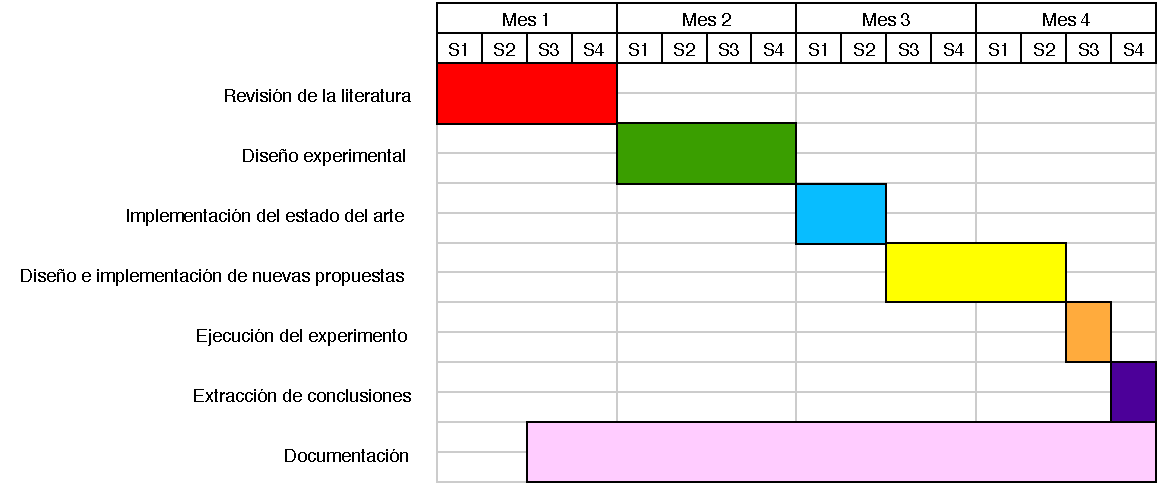
\includegraphics[scale=0.6]{imagenes/cronograma.pdf}
	\caption{Cronograma ilustrativo de la planificación del estudio.}
	\label{cronograma}
\end{figure}
\chapter{Revisión de la literatura: estado del arte}

En este capítulo se expondrá una revisión de los estudios y propuestas más innovadoras relacionadas con los \textbf{sistemas de recomendación a grupos}, y en particular, de aquellos orientados al ámbito de las películas. Se comenzará haciendo un breve inciso sobre cuándo y cómo se originaron los sistemas de recomendación, así como la particularidad de aquellos específicos de recomendación a grupos. Después se tratará su evolución hasta nuestros días, realizando un comentario analítico acerca de lo que han supuesto los sistemas de recomendación y cómo se trasladan actualmente dichos sistemas a situaciones cotidianas, con algunos claros ejemplos que todo el mundo utiliza. Entre ellos se destacarán los que abarcan la \textbf{recomendación de películas}, como tema principal del estudio. Por último, se mencionarán algunos de los sistemas de recomendación de películas a grupos más actuales, eligiendo además el que será tomado como referencia para la experimentación como representante del estado del arte de estos recomendadores.

Queda ya muy atrás el primer sistema de recomendación de la historia, que vio la luz en 1992, cuando Goldberg et al. (1992) presentaron su artículo \textit{``Using collaborative filtering to Weave an Information tapestry''} \cite{tapestry-goldberg}. En este trabajo se acuña por primera vez el término \textbf{``filtrado colaborativo''} (en inglés, \textit{collaborative filtering}), refiriéndose así a la técnica que permite filtrar elementos a un usuario basándose en lo que otros usuarios han opinado de él anteriormente. Esta técnica sienta las bases de los sistemas de recomendación, y aún a día de hoy se encuentra presente en la mayoría de ellos. La otra alternativa al filtrado colaborativo es el \textbf{filtrado basado en contenido} (en inglés, \textit{content-based filtering}). Esta técnica no tiene en cuenta las valoraciones que otros usuarios han dado a los elementos del sistema, sino que se limita a comparar los elementos por características y recomendar aquellos similares. En este experimento, sin embargo, se tratarán únicamente métodos que utilizan el filtrado colaborativo.

Una vez se hubo contemplado el vasto rango de opciones que albergaban los sistemas de recomendación, a través de numerosos trabajos y estudios, se contempló la posibilidad de recomendar ya no solo a individuos, sino a grupos de personas. Se trataba de una situación a la que una sociedad podía enfrentarse en multitud de facetas, y que sin duda merecía la pena explorar. La pionera, y una de las más famosas y reconocidas propuestas sobre este tema, fue \textbf{PolyLens} \cite{polylens}. En esta publicación de 2001, O'Connor et al. plantearon \textbf{un sistema de recomendación de películas para grupos}, derivado de la base de datos de valoraciones de películas \textbf{MovieLens}, en la que varios trabajos anteriores se habían fundado. Este sistema abrió la veda de un nuevo subgrupo dentro de la ya amplia categoría de sistemas de recomendación.

Como se ha comentado anteriormente, las recomendaciones a películas han levantado mucho interés desde el primer momento. El contenido de ocio audiovisual, junto a los catálogos de tiendas \textit{online}, son los casos de mayor demanda en cuanto a sistemas de recomendación en la sociedad actual. Plataformas como \textbf{Netflix}, \textbf{Spotify} o \textbf{HBO} son ejemplos de los primeros, que utilizan estos sistemas para tratar de mantener al usuario satisfecho ofreciéndole nuevo contenido que sea similar al que hayan visto. Por su parte, \textbf{Amazon} o \textbf{AliExpress} son ejemplos de los segundos, grandes plataformas que dan cabida a todo tipo de productos y que son capaces de recomendar a sus clientes otros productos similares a los que están buscando. Gracias al sistema de recomendación pertinente, incluso consiguen ofrecer nuevos artículos que detectan que el usuario puede querer comprar, basándose en lo que anteriormente ha buscado o comprado.

Tal fue el impacto de los sistemas de recomendación que la propia plataforma Netflix lanzó en 2006 lo que se conocería como el \textbf{Netflix Prize} \cite{netflix-prize}, una competición de sistemas que, basándose únicamente en el filtrado colaborativo (no conociendo datos adicionales sobre películas ni sobre usuarios, solamente las valoraciones que estos habían dado a cada película) fueran capaces de predecir acertadamente dichas valoraciones. El objetivo principal era superar al por aquel entonces actual sistema de recomendación de Netflix, conocido como \textbf{Cinematch}, ofreciendo un premio de 1 millón de dólares a aquel sistema capaz de superarlo en un 10\%. Adicionalmente, como la competición se estimaba que duraría hasta 2011, se concedería un premio anual de 50.000 dólares al método ganador al final de cada año.

Tras varios tira y afloja entre algunos equipos, e incluso agrupaciones entre equipos para forjar mejores ideas juntos, finalmente en 2009 el equipo \textit{'BellKor's Pragmatic Chaos'} se alzó ganador y recibió el gran premio \cite{netflix-prize-winner}, superando al algoritmo anterior por 10.05\%. De esta forma tan original Netflix cambió su sistema de recomendación promoviendo una iniciativa de investigación en este campo, y por supuesto previendo que este avance en su algoritmo les serviría para incrementar la satisfacción de sus clientes, y por ende, para aumentar su valor de mercado.

Tras haber sido puestos en el panorama de investigación con casos como el Netflix Prize y el evidente aumento de su uso conforme las nuevas tecnologías se han vuelto más accesibles para la sociedad, los sistemas de recomendación han contemplado un gran abanico de variedades: algunos más enfocados a la materia que recomendar (por ejemplo, sistemas de recomendación de música o de películas), otros enfocados al tipo de usuario (sistemas de recomendación individual o a grupos) e incluso algunos cuyo propósito no es solamente obtener el mejor resultado (sistemas de recomendación explicativos que sirvan de apoyo a una decisión).

Como el objetivo de este trabajo es orientarse en recomendación a películas para grupos de usuarios, la búsqueda en la literatura de algoritmos que apoyasen el estudio se focalizó en estos dos grandes campos, analizando algunos algoritmos de la última década. La recomendación a grupos ha avanzado a muchos niveles desde la presentación de PolyLens, y ahora existen varios frentes abiertos en investigación sobre este tema.

Uno de las primeras fuentes que se recopilaron sobre los sistemas de recomendación a grupos, y que han servido a este estudio para obtener información general sobre los mismos, es el capítulo de Masthoff en el \textit{Recommender Systems Handbook} de 2011 \cite{masthoff-handbook}, donde hace un repaso a los campos de investigación abiertos de los que se hablaba en el párrafo anterior, y realiza un análisis sobre los pasos a seguir en adelante. Masthoff sienta en primer lugar los motivos por los que es necesario contar con sistemas de recomendación a grupos frente a la recomendación individual que ya se había trabajado más de una década. Aporta una detallada recopilación de las estrategias de agregación que utilizaban los sistemas de recomendación a grupos más interesantes de la época, como el ya mencionado PolyLens \cite{polylens}, el sistema MusicFX \cite{musicfx} que determina la emisora de radio que suena de fondo en un gimnasio en función de los gustos de la gente que haya ejercitándose en ese momento, o el sistema Intrigue \cite{intrigue} que ayuda a grupos de turistas a decidir qué visitar, entre otros. A continuación explica cómo se pueden aplicar los algoritmos de recomendación a grupos para usuarios individuales, dando a entender que estos algoritmos son reutilizables dependiendo del contexto en el que se necesiten. Termina planteando una serie de retos a los que los sistemas de recomendación a grupos se enfrentaban en aquel momento: aportar explicaciones a las recomendaciones propuestas, profundizar en el ``problema del inicio frío'' para grupos de usuarios o recomendar ítems en un determinado orden.

En el contexto de las recomendaciones ordenadas podrían englobarse los \textbf{rankings}, que es hacia donde han evolucionado los recomendadores individuales en las principales páginas. Es habitual no limitarse a recomendar un único ítem a un usuario, lo que propicia que se investigue en recomendar series de elementos dándoles un determinado orden (por supuesto, se quiere colocar en primer lugar aquel que se prediga que va a tener más aceptación).


%
%%\chapter{Conclusiones y Trabajos Futuros}
%
%
\nocite{*}
\bibliography{bibliografia/bibliografia}\addcontentsline{toc}{chapter}{Bibliografía}
\bibliographystyle{unsrt}
%
%\appendix
%\input{apendices/manual_usuario/manual_usuario}
%%\input{apendices/paper/paper}
%\input{glosario/entradas_glosario}
% \addcontentsline{toc}{chapter}{Glosario}
% \printglossary
\chapter*{}
\thispagestyle{empty}

\end{document}
